\section{Knot coloring}

Let $R$ be any commutative ring with identity, let $M$ be a module with one generator and $\phi:M^3\to M$ be a homomorphism such that for every $m\in M$
%$M$ be any \textbf{\color{red}finitely generated} $R$-module and $\phi:M^3\to M$ be a homomorphism such that for every $m\in M$ 
\begin{equation}\label{phi allows for trivial colorings}
  \phi(m,m,m)=0.
\end{equation}
Notice that if $\phi(u,i,o)=au+bi+co$, then aforementioned equality demands that $(a+b+c)\in \ann(M)$.

Take $K$ to be any knot with diagram $D$ with $s$ arches and $x$ crossings.

\begin{lemma}
  For diagrams of knots other than $0_1$, the number of segments $s$ is equal to the number of crossings $x$.
\end{lemma}

\begin{proof}
  Every crossing has $2$ arcs that go below it and every arc has two bottom ends that are created when this segment disappears below another segment. Thus 
  $$2\cdot \#\text{arches} = \#\text{bottom ends} = 2\cdot \#\text{crossings}.$$
\end{proof}

\begin{definition}\label{coloring definition primitive}
  We say that $C\subseteq M^s$ is a \emph{coloring module} of the diagram $D$ with elements from $M$ if it 
  \begin{enumerate}
    \item {\color{orange}has $s$ generators, each corresponding to one arc of the diagram}, 
    \item and for every $u, i, o\in C$ that correspond to arcs meeting in one crossing, $\phi(u,i,o)=0$.
  \end{enumerate}
  \begin{center}
    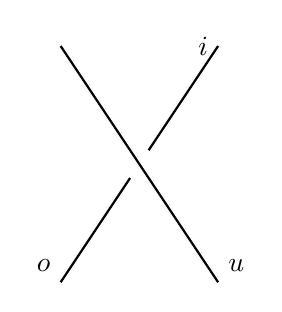
\begin{tikzpicture}
      \draw[thick] (0,0) node[above left] {$o$} --(2, 3) node [left] {$i$};
      \fill[white] (1, 1.5) circle (6pt);
      \draw[thick] (0, 3)--(2, 0) node[above right] {$u$};
    \end{tikzpicture}
  \end{center}
\end{definition}

Notice that condition stated in \cref{phi allows for trivial colorings} makes it possible to color every diagram trivially, that is by assigning the same element of $M$ to every arc of $D$.

Approach to coloring taken in \cref{coloring definition primitive} gives a lot of information about coloring with elements of one specific module $M$ and if one was to change the module to some $M'\neq M$, almost all information gathered for previous coloring would be now ineffectual. Consider the following example.
%it is rather difficult to extrapolate it for other modules. Consider the following example.
%it is rather difficult to use it for other modules. Consider the following example.

\begin{example}
  Take $R=\Z$ with $\phi(x, y, z)=2x-y-z$ and consider the trefoil knot $3_1$. If we take $M=\Z$ then $K$ admits only the trivial coloring module: 
  $$C_M=\{(x, x, x)\;:\;x\in\Z\}.$$ 
  However, if we take $M'=\Z_3$ then there exists a non-trivial coloring like the one presented in \cref{trefoil knot diagram 1}.
  \begin{figure}[h]\centering
    \begin{tikzpicture}[bgnd/.style={circle, fill=white, draw=white}]
       \begin{knot}[
         consider self intersections,
         flip crossing=2,
         clip width=20,
         ]
         \strand[thick]
         (90:3) to[out=180,in=-120,looseness=2]
         (-30:3) to[out=60,in=120,looseness=2]
         (210:3) to[out=-60,in=0,looseness=2] (90:3);
       \end{knot}

       \node[bgnd] at (90:3) {$0$};
       \node[bgnd] at (-30:3) {$1$};
       \node[bgnd] at (210:3) {$2$};
  \end{tikzpicture}
 \caption{The trefoil knot $3_1$ does not allow for nontrivial coloring over $M=\Z$ but it is possible to color it with $M=\Z_3$.\label{trefoil knot diagram 1}}
\end{figure}
\end{example}

Another approach to defining coloring module of a knot diagram $D$ would be by starting with identifying arches with generators $(0,..., 1, ..., 0)$ of $M^s$. Then, we might define a homomorphism
$$f:M^s\to M^x$$
such that arches building one crossing follow rules set by $\phi$.

% We might want to start defining coloring by defining a homomorphism
% $$f:M^s\to M^x$$
% which identifies coordinates with arcs in $D$ and follows $\phi$ on triples of coordinates that build one crossing. 

\begin{definition}\label{coloring definition as kernel}
  Module $\ker f$ is a coloring module of diagram $D$ with elements of $M$.
\end{definition}

Henceforth, we will call $f$ described above a \textbf{coloring homomorphism} for chosen $R$, $M$ and $\phi$.

\begin{corollary}\label{rownowaznosc definicji}
  \Cref{coloring definition primitive} and \cref{coloring definition as kernel} are equivalent for one dimensional modules.
\end{corollary}

\begin{proof}
  {\large\color{red}TO DO}
\end{proof}

Despite the fact that it is the kernel of $f$ that contains colorings, examining the coloring homomorphism itself gives more information about diagram $D$. We might consider $f$ as a $s\times s$ matrix and if $R$ is a PID module, then we can represent this matrix in Smith's normal form. 
%This representation contains information about the kernel over the specific module $M$ and ring $R$ but also shows how to change $M$ and even $R$ to obtain a different coloring.

\begin{proposition}
  Let $A$ be the Smith's normal form of $f$. Columns of $A$ comprised only of zeros and zero divisors contribute to the coloring module. %Moreover, non-unit elements that appear on the diagonal hint at what other colorings are admissible.
\end{proposition}

\begin{proof}
  An immediate result of \cref{rownowaznosc definicji}. The second part 
%  {\large\color{red}TUTAJ WOGÓLE POTRZEBA COKOLWIEK DOWODZIĆ?}
\end{proof}

%Furthermore, if $R$ is a Noetherian ring, then every finitely generated module is a quotient of a free module with the same number of generators. Thus, taking $M$ to be any finitely generated module over $R$ gives us information about coloring with any other module with equal number of generators.

{\color{blue}
If $R$ is a Noetherian ring, then every finitely generated module is a quotient of a free module with the same number of generators. Thus, we might want to take $M$ to be a finitely generated free $R$-module rather than any one dimensional $R$-module. This allows us to send $M$ to any other $R$-module with at most $\dim (M)$ generators to obtain a different coloring.
}

%Usually, it is the irreversible elements from the diagonal of Smith's form $f$ that hint at what colorings are admisible. Consider the following example.

The nonzero elements that appear on the diagonal of the normal form of the coloring homomorphism hint at what colorings over the ring $R$ are admissible. Consider the following example.

\begin{example}\label{ex2}
  As before, take $R=\Z$ and $\phi(x, y, z)=2x-y-z$. Taking $M=\Z$ we have $f:\Z^3\to \Z^3$ for trefoil knot to be a matrix
  $$ 
  \begin{pmatrix}
    2 & -1 & -1 \\ 
    -1 & 2 & -1 \\ 
    -1 & -1 & 2
  \end{pmatrix}
  $$ 
  with Smith's normal form
  $$
  \begin{pmatrix}
    -1 & 0 & 0 \\ 
    0 & 3 & 0\\ 
    0 & 0 & 0
  \end{pmatrix}
  $$
  The normal form of the coloring homomorphism contains a $3$, hinting that $\Z/(3)$ allows for a non-trivial coloring. Send $M=\Z$ to $M'=\Z_3$ by taking all coefficient modulo $3$ to obtain the new Smith's normal form of $f$ to be
  $$
  \begin{pmatrix}
    -1 & 0 & 0 \\ 
    0 & 0 & 0\\ 
    0 & 0 & 0
  \end{pmatrix}
  $$
  which informs about the nontrivial coloring presented in \cref{trefoil knot diagram 1}, that was not allowed over $\Z$.
\end{example}

